\documentclass[twocolumn, amsmath, amsfonts, amssymb, trackchanges]{aastex62}
\usepackage{mathtools}
\usepackage{natbib}
\usepackage{bm}
\newcommand{\vdag}{(v)^\dagger}
\newcommand\aastex{AAS\TeX}
\newcommand\latex{La\TeX}


\newcommand{\Div}[1]{\ensuremath{\nabla\cdot\left( #1\right)}}
\newcommand{\DivU}{\ensuremath{\nabla\cdot\bm{u}}}
\newcommand{\angles}[1]{\ensuremath{\left\langle #1 \right\rangle}}
\newcommand{\td}[1]{\ensuremath{\widetilde{#1}}}
\newcommand{\KSstat}[1]{\ensuremath{\overline{\text{KS}(#1)}}}
\newcommand{\grad}{\ensuremath{\nabla}}
\newcommand{\RB}{Rayleigh-B\'{e}nard }
\newcommand{\stressT}{\ensuremath{\bm{\bar{\bar{\Pi}}}}}
\newcommand{\lilstressT}{\ensuremath{\bm{\bar{\bar{\sigma}}}}}
\newcommand{\nrho}{\ensuremath{n_{\rho}}}
\newcommand{\approptoinn}[2]{\mathrel{\vcenter{
	\offinterlineskip\halign{\hfil$##$\cr
	#1\propto\cr\noalign{\kern2pt}#1\sim\cr\noalign{\kern-2pt}}}}}

\newcommand{\appropto}{\mathpalette\approptoinn\relax}
\newcommand{\pro}{\ensuremath{\text{Ro}_{\text{p}}}}
\newcommand{\con}{\ensuremath{\text{Ro}_{\text{c}}}}

\usepackage{color}
\newcommand{\gv}[1]{{\color{blue} #1}}

%% Tells LaTeX to search for image files in the 
%% current directory as well as in the figures/ folder.
\graphicspath{{./}{figs/}{../tex/figs/}}


\received{\today}
\revised{\today}
\accepted{??}%\today}
\submitjournal{ApJ}

%%%%%%%%%%%%%%%%%%%%%%%%%%%%%%%%%%%%%%%%%%%%%%%%%%%%%%%%%%%%%%%%%%%%%%%%%%%%%%%
%% TITLE & AUTHORS
\shorttitle{Stratified Thermals}
\shortauthors{Anders et al.}

\begin{document}
\title{Entrainment of low Mach number thermals in stratified domains}

\correspondingauthor{Evan H. Anders}
\email{evan.anders@colorado.edu}

\author[0000-0002-3433-4733]{Evan H. Anders}
\affil{Dept. Astrophysical \& Planetary Sciences, University of Colorado -- Boulder, Boulder, CO 80309, USA}
\affil{Laboratory for Atmospheric and Space Physics, Boulder, CO 80303, USA}
\author[0000-0002-7635-9728]{Daniel Lecoanet}
\affil{Stuff}
\author[0000-0001-8935-219X]{Benjamin P. Brown}
\affil{Dept. Astrophysical \& Planetary Sciences, University of Colorado -- Boulder, Boulder, CO 80309, USA}
\affil{Laboratory for Atmospheric and Space Physics, Boulder, CO 80303, USA}


\begin{abstract}
\end{abstract}

\keywords{hydrodynamics --- turbulence --- entrainment}

%%%%% Body of the paper
%%%%%%%%%%%%%%%%%%%%%%%%%%%%%%%%%%%%%%%%%%%%%%%%%%%%%%%%%%%%%%%%%%%%%
%% INTRODUCTION
\section{Introduction}
\label{sec:intro}
(Para 1) Brief intro to solar convective conundrum.

(Para 2) Entropy rain history and expansion by Axel

(Para 3) Boussinesq thermals and their filling factor vs. depth.

(Para 4) What we're doing here, how it fits into this context.

(Para 5) Standard last paragraph of an intro?

%%%%%%%%%%%%%%%%%%%%%%%%%%%%%%%%%%%%%%%%%%%%%%%%%%%%%%%%%%%%%%%%%%%%%%%%%%%%%%
%% THEORY SECTION
\section{Theory}
\label{sec:theory}

\subsection{Phenomenological description of thermal evolution}
The initial conditions of the thermals studied in this work are spherical
entropy perturbations with zero initial velocity, as depicted in 
Fig.~\ref{fig:evolution_colormeshes}a. Buoyant forces cause these perturbations
to fall and develop into vortex rings, as depicted in 
Figs.~\ref{fig:evolution_colormeshes}c-f.

\begin{figure*}[t!]
    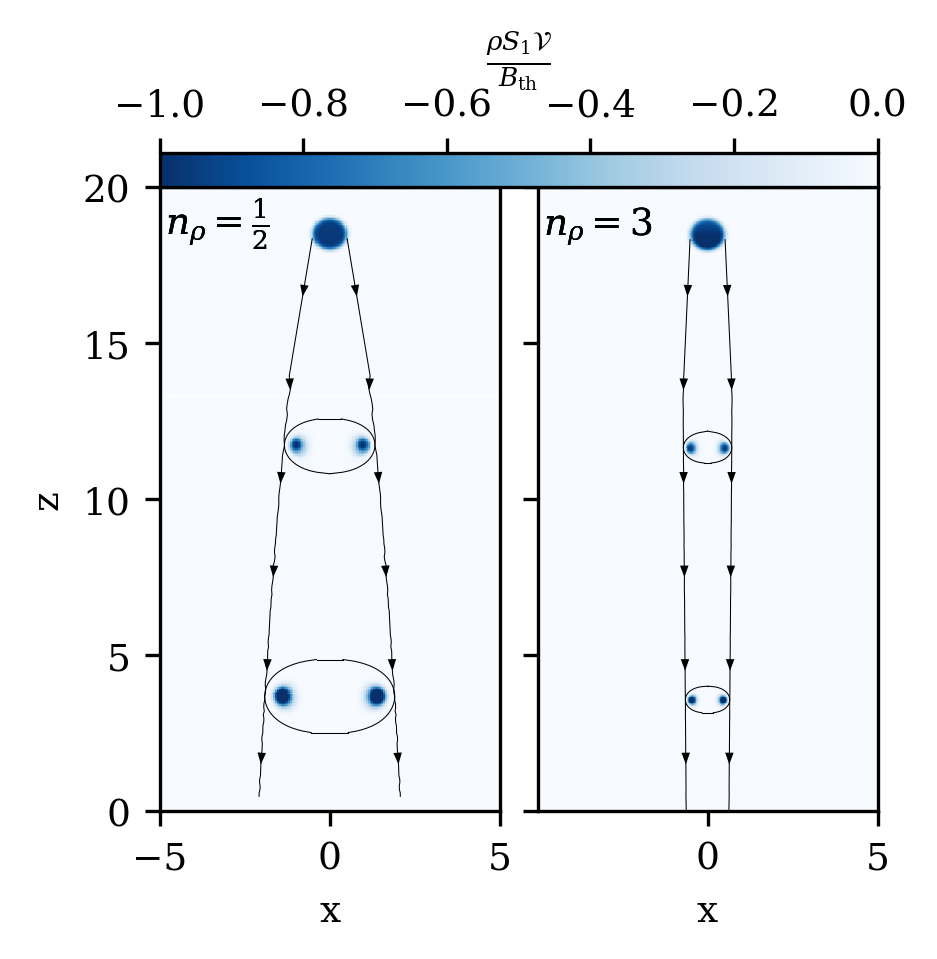
\includegraphics[width=\textwidth]{evolution_colormeshes.png}
    \caption{
    \label{fig:evolution_colormeshes} }
\end{figure*}


\subsection{Theoretical description of thermal evolution}
The evolution of thermals as buoyant vortex rings has been well described in
the unstratified, Boussinesq limit for decades (as early as e.g., CITE, and
see \citet{lecoanet&jeevanjee2018} for other sources). Buoyant motions 
in the atmospheres of stars and planets are generally large enough to feel the
atmospheric stratification, and therefore a more thorough tratment of the
evolution of thermals in stratified domains is required to understand the nature
of thermal entrainment in nature.

In this work, we focus on the non-dissipative, low Mach number regime, 
in which the ideal anelastic equations are a decent approximation to the fully
compressible equations. In this regime, the buoyancy is directly proportional to the
specific entropy. In the absence of diffusion, or in the limit where diffusivities
are sufficiently small, the volume-integrated total entropy is constant,
\begin{equation}
B \equiv \int_{\mathcal{V}} \rho\, s\, dV = \text{const},
\end{equation}
where $s = c_V \ln T - R \ln\rho$ is the specific entropy, with $c_V$ the
specific heat at constant volume and $R$ the ideal gas constant.

In a stratified domain, the hydrodynamic impulse is defined
\citet{shivamoggi2010},
\begin{equation}
\bm{I} = \frac{1}{2}\int_{\mathcal{V}} \bm{x}\times(\grad\times(\rho\bm{u}))dV,
\end{equation}
where $\bm{x}$ is the position vector, $\bm{u}$ is vector velocity, $\rho$ is density,
and $\mathcal{V}$ is the volume being integrated over. Furthermore, changes in the impulse
can be expressed
\begin{equation}
\frac{\partial\bm{I}}{\partial t} = \int_{\mathcal{V}}\frac{\partial}{\partial t}(\rho \bm{u})dV
= B\hat{z} + S,
\end{equation}
where $S$ is a combination of surface terms that disappears upon appropriate boundary conditions
on $\mathcal{V}$ \citep{shivamoggi2010}. As we have assumed that the buoyancy, $B$, is constant,
we can straightforwardly integrate
\begin{equation}
I_z = B t + I_0,
\end{equation}
for some constant $I_0$.

(need to work through this section carefully).
Assuming an adiabatically stratified atmosphere in
hydrostatic equilibrium, the vertical momentum equation is
\begin{equation}
 = - \partial_z \varpi +  g\frac{S_1}{c_P},
\label{eqn:buoyancy}
\end{equation}
where $w$ is vertical velocity, $S_1$ is specific entropy, $\varpi$ is the reduced pressure,
$D/Dt = \partial_t + (\bm{u}\cdot\grad)$ is the (eulerian? lagrangian?)
derivative, $g$ is gravity, and $c_P$ is the specific heat at constant pressure.
In the anelastic approximation, the density stratification is constant in time. 
OH GOD I DON'T KNOW THIS MATH WELL MAGIC MAGIC MAGIC.
By doing magic, we arrive at
\begin{equation}
P_z = \beta B t + P_0.
\end{equation}

Under the assumption that the thermal develops into a thin-core 
propagating vortex ring whose vortex core is radius $r$ away from the axis of symmetry, 
the impulse can be approximated as $I_z \approx \pi \rho r^2 \Gamma$, where 
$\Gamma$ is the circulation of the thermal vortex, which we assume to be constant. 
Rearranging, we find our first result,
\begin{equation}
r = \sqrt{\frac{B t + I_0}{\pi\rho\Gamma}}.
\label{eqn:r_theory}
\end{equation}
In the limit where $\rho \rightarrow \text{constant}$, as in the Boussinesq regime,
we retrieve the $r \propto \sqrt{t}$ scaling found in the Boussinesq regime by
\citet{lecoanet&jeevanjee2018}. We find that the inclusion of stratification adds the
additional complexity of $r \propto \rho^{-1/2}$, such that downward-propogating 
vortex rings (as studied here) will not entrain to the same degree as boussinesq thermals,
and upward-propogating rings will entrain more.

We further assume that the volume-integrated momentum, $P_z \approx \rho V w_{th}$,
where $w_{th}$ is the vertical velocity of the thermal as a whole, and the volume
of the fluid region propogating with the thermal is a spheroid, $V = V_0 r^3$, for
some constant $V_0$. Plugging Eqn.~\ref{eqn:r_theory} into this approximation, we
find that
\begin{equation}
\rho^{-1/2}w = \left(\frac{(\pi\Gamma)^{3/2}}{V_0}\right)\frac{\beta B t + M_0}{(B t + I_0)^{3/2}}.
\end{equation}
Substituting $w = dz/dt$ and $\tau \equiv (Bt + I_0)/\Gamma$, We retrieve
\begin{equation}
\frac{dz}{\sqrt{\rho(z)}} 
= \left(\frac{\pi^{3/2}\Gamma}{V_0}\right)
\left(\beta\Gamma\tau^{-1/2} + [M_0 - \beta I_0]\tau^{-3/2}\right)d\tau.
\end{equation}
If the atmospheric stratification in which the thermal is falling is known, this
result can be straightforwardly integrated with $\rho(z)$ plugged in in order to
find the position of the thermal versus time. While we will leave this result
general for now, we will plug in our polytropic stratification at the end of
section \ref{sec:experiment}, and show that the resulting expression does a
good job of explaining the evolution of thermals in these atmospheres in
section \ref{sec:results}.

%%%%%%%%%%%%%%%%%%%%%%%%%%%%%%%%%%%%%%%%%%%%%%%%%%%%%%%%%%%%%%%%%%%%%%%%%%%%%%%
%% EXPERIMENT SECTION
\section{Experiment} 
\label{sec:experiment}

\subsection{Polytropic Atmospheres}
We study an ideal gas whose equation of state is $P = \rho T$ and whose stratification
is a perfectly adiabatic polytrope,
\begin{gather}
T_0 = 1 + (\grad_{\text{ad}})(z - L_z) \\
\rho_0 = T_0^{m_{\text{ad}}},
\end{gather}
where $m_{\text{ad}} = (\gamma-1)^{-1}$, and where the adiabatic 
temperature gradient is $\grad_{\text{ad}} = - g / c_P$.

\subsection{Anelastic Equations}
The anelastic equations are \citep{lecoanet&all2014},
\begin{gather}
\td{\grad}\cdot\td{\bm{u}} = -\td{w}\partial_{\tilde{z}} \ln\rho_0 \\
\frac{D \td{\bm{u}}}{D \td{t}} = -\td{\grad} \td{\varpi} + g\frac{\td{S_1}}{c_P}\hat{z} + \frac{1}{\rho_0}\td{\grad}\cdot\left(\mu\td{\lilstressT}\right) \\
\frac{D \td{S_1}}{D\td{t}} = \frac{1}{\rho c_P}\td{\grad}\cdot\left(\kappa T_0 \td{\grad} \td{S_1}\right) + \frac{\mu}{\rho_0 T_0}\td{\sigma_{ij}}\partial_{\td{x_i}}\td{u_j}.
\end{gather}
where $D/D\td{t} = \partial/\partial \td{t} + \td{\bm{u}}\cdot\td{\grad}$ and the viscous stress tensor is
\begin{equation}
\td{\sigma_{ij}} = \left(\partial_{\td{x_i}}\td{u_j} + \partial_{\td{x_j}}\td{u_i} - \frac{2}{3}\delta_{ij}\td{\grad}\cdot\td{\bm{u}}\right).
\end{equation}

We nondimensionalize these equations as in \citet{lecoanet&jeevanjee2018} such that
the length scale is the diameter of the thermal and the velocity scale is the freefall
velocity,
\begin{equation}
\begin{split}
\td{\grad}\rightarrow(\td{L}_{th}^{-1})\grad, \qquad&
\td{S}_1 \rightarrow(\Delta\td{S})S_1,\\
\td{\bm{u}} \rightarrow (\td{u}_{th})\bm{u}, \qquad&
\td{\varpi} \rightarrow (\td{u}_{th}^2)\varpi,\\
\partial_{\tilde{t}} \rightarrow (\td{u}_{th}/\td{L}_{th})\partial_t,\qquad&
\end{split}
\end{equation}
with
\begin{equation}
\tilde{u}_{th}^2 = \frac{g \tilde{L}_{th} \Delta \tilde{s}}{c_P}, \qquad
\text{Re}_{\text{ff}} = \frac{\tilde{u}_{th} \tilde{L}_{th}}{\nu}, \qquad
\text{Pr}_{\text{ff}} = \frac{\tilde{u}_{th} \tilde{L}_{th}}{\chi}.
\end{equation}
The resulting equations are very similar to the boussinesq equations,
\begin{gather}
\DivU = -w \partial_z \ln\rho_0, \\
\begin{split}
\partial_t \bm{u} + \bm{u}\cdot\grad\bm{u} = \\
- \grad \varpi + S_1\hat{z} 
+ \frac{1}{\text{Re}_{\text{ff}}}\left[\grad^2 \bm{u} + \frac{1}{3}\grad(\DivU)\right] 
\end{split}\\
\begin{split}
\partial_t S_1 + \bm{u}\cdot\grad S_1 = \\
\frac{1}{\text{Re}_{\text{ff}}}\left(\frac{1}{\text{Pr}_{\text{ff}}\rho_0c_P }[\grad^2 S_1 + \partial_z\ln T_0 \cdot\partial_z S_1]\right.\\\left.
+ \frac{-(\grad_{ad})}{\rho_0 T_0}\sigma_{ij}\partial_{x_i}u_j \right)
\end{split}
\end{gather}

\subsection{Fully Compressible Equations}
The fully compressible equations, under the same assumptions as above, are
\begin{gather}
\frac{D \ln\rho}{Dt} + \DivU = 0 \\
\frac{D \bm{u}}{D t} = -\grad T - T\grad\ln\rho - g\hat{z} + \frac{1}{\rho}\grad\cdot\left(\mu\lilstressT\right) \\
\frac{D T}{Dt} + (\gamma-1)T\DivU  = \frac{1}{\rho c_V}\grad\cdot\left(\kappa \grad T\right) + \frac{\mu}{\rho c_V}\sigma_{ij}\partial_{x_i}u_j.
\end{gather}

\subsection{Initial Conditions}
We set the initial specific entropy perturbation as
\begin{equation}
S_1 = - A(1 - \text{erf}\left(\frac{r - r_{th}}{\delta}\right))/2,
\end{equation}
where in the FC cases $A = 10^{-4}$ and in the nondimensionalized AN cases,
$A = 1$. Here, $r = \sqrt{x^2 + y^2 + (z - z_0)^2}$, where $z_0 = Lz - 3*r_{th}$,
and $r_{th} = Lz/40$ is the radius of the thermal.

In the fully compressible equations, it is essential that the initial conditions be in pressure
equilibrium such that the low mach number nature of the thermal can be studied. In order to 
achieve this pressure balance, we set
\begin{equation}
\ln\rho_1 = S_1/c_P, \qquad T_1 = T_0(e^{-\ln\rho_1} - 1).
\end{equation}


\subsection{Solution for thermal evolution in a Polytrope}


\subsection{Verification of 2D Anelastic approximation}
blah blah blah comparison of 2D and 3D blah blah blah. z v t, r v z, w v z. Also side-by-side
pictoral comparison with diff.


%%%%%%%%%%%%%%%%%%%%%%%%%%%%%%%%%%%%%%%%%%%%%%%%%%%%%%%%%%%%%%%%%%%%%%%%%%%%%%%
%% RESULTS SECTION
\section{Results}
\label{sec:results}
Picture of a big old grid of z v t, r v z, w v z.

Pretty picture showing thermal evolution (comparing low and high stratification).

Verification of theory by simulations

Table of found parameters for the fits

Two regimes: stalling and falling.


%%%%%%%%%%%%%%%%%%%%%%%%%%%%%%%%%%%%%%%%%%%%%%%%%%%%%%%%%%%%%%%%%%%%%%%%%%%%%%%
%% CONCLUSION SECTION
\section{Discussion}
\label{sec:discussion}
Wild speculation about extensions to the solar regime. Do things on the sun shrink
to the point where they viscously dissipate?

Talk about what would happen if we were to study up-thermals.

Extensions, and the fact that we trust these results will likely hold in the solar regime.



\begin{acknowledgements}
This work was supported by NASA Headquarters under the NASA Earth and Space
Science Fellowship Program -- Grant 80NSSC18K1199.
This work was additionally supported by  NASA LWS grant number NNX16AC92G.  
Computations were conducted 
with support by the NASA High End Computing (HEC) Program through the NASA 
Advanced Supercomputing (NAS) Division at Ames Research Center on Pleiades
with allocation GID s1647.
\end{acknowledgements}

\appendix
\section{Thermal Tracking}
\label{appendix:tracking}

\section{Table of Simulations}
\label{appendix:table}

%\begin{deluxetable*}{c c c c c c c c c c c c c c c}
%\tabletypesize{\footnotesize}
%\caption{Table of simulation information
%\label{table:simulation_info}
%}
%\tablehead{																																															
%\colhead{Ra$_{\text{top}}$}	&	\colhead{Ta$_{\text{top}}$}	&	\colhead{Ro$_{\text{p, top}}$}	&	\colhead{Ra$_{\text{mid}}$}	&	\colhead{Ta$_{\text{mid}}$}	&	\colhead{Ro$_{\text{p, mid}}$}	&	\colhead{\con}	&	\colhead{$\mathcal{S}$}	&	\colhead{$L_x/L_z$}	&	\colhead{(nz,	nx,	ny)}	&					\colhead{Ro}      	&	\colhead{Re$_{\parallel}$} 	&	\colhead{Re$_{\perp}$}	&	\colhead{Nu}      	}														
%\startdata																																															
%\multicolumn{3}{l}{\textbf{Constant \pro$\,$, path III}}\\
%1.8	$\times 10^{	5	}$	&	4.1	$\times 10^{	7	}$	&	0.60	&	1.4	$\times 10^{	7	}$	&	3.0	$\times 10^{	9	}$	&	1.03	&	0.067	&	1.1	&	0.51	&	(256,		32,		32)	&	0.015	&	19.4	&	2.5	&	1.2	\\				
%1.2	$\times 10^{	9	}$	&	5.2	$\times 10^{	12	}$	&	0.60	&	9.2	$\times 10^{	10	}$	&	3.8	$\times 10^{	14	}$	&	1.03	&	0.015	&	3.0	&	0.07	&	(2048,		64,		64)	&	0.026	&	1771	&	32.0	&	15.4	\\				
%5.2	$\times 10^{	2	}$	&	4.6	$\times 10^{	3	}$	&	0.96	&	3.8	$\times 10^{	4	}$	&	3.4	$\times 10^{	5	}$	&	1.64	&	0.333	&	1.13	&	2.28	&	(64,		64,		64)	&	0.074	&	4.2	&	2.5	&	1.2	\\				
%3.8	$\times 10^{	8	}$	&	3.1	$\times 10^{	11	}$	&	0.96	&	2.8	$\times 10^{	10	}$	&	2.3	$\times 10^{	13	}$	&	1.64	&	0.035	&	6.0	&	0.12	&	(2048,		64,		64)	&	0.129	&	3906	&	113	&	66.9	\\				
%7.9	$\times 10^{	1	}$	&	1.0	$\times 10^{	2	}$	&	1.58	&	5.8	$\times 10^{	3	}$	&	7.4	$\times 10^{	3	}$	&	2.70	&	0.888	&	1.56	&	4.44	&	(64,		64,		64)	&	0.303	&	4.4	&	4.9	&	1.7	\\				
%1.4	$\times 10^{	7	}$	&	9.7	$\times 10^{	8	}$	&	1.58	&	1.0	$\times 10^{	9	}$	&	7.2	$\times 10^{	10	}$	&	2.70	&	0.119	&	10.0	&	0.30	&	(512,		128,		128)	&	0.376	&	1257	&	94.9	&	40.1	\\				
%\hline																																															
%\multicolumn{3}{l}{\textbf{Constant \con$\,$, path II}}\\
%8.6	$\times 10^{	4	}$	&	8.6	$\times 10^{	6	}$	&	0.74	&	6.3	$\times 10^{	6	}$	&	6.3	$\times 10^{	8	}$	&	1.26	&	0.1	&	1.47	&	0.68	&	(128,		128,		128)	&	0.051	&	40.2	&	6.7	&	2.2	\\				
%2.6	$\times 10^{	6	}$	&	2.6	$\times 10^{	8	}$	&	1.13	&	1.9	$\times 10^{	8	}$	&	1.9	$\times 10^{	10	}$	&	1.93	&	0.1	&	4.64	&	0.39	&	(256,		512,		512)	&	0.27	&	565	&	53.2	&	33.3	\\				
%1.4	$\times 10^{	3	}$	&	1.6	$\times 10^{	4	}$	&	1.01	&	1.1	$\times 10^{	5	}$	&	1.2	$\times 10^{	6	}$	&	1.72	&	0.3	&	1.47	&	1.90	&	(64,		128,		128)	&	0.124	&	11.3	&	5.4	&	1.8	\\				
%1.1	$\times 10^{	6	}$	&	1.2	$\times 10^{	7	}$	&	2.29	&	7.8	$\times 10^{	7	}$	&	8.6	$\times 10^{	8	}$	&	3.93	&	0.3	&	14.7	&	0.65	&	(192,		384,		384)	&	0.808	&	529	&	83.5	&	27.3	\\				
%5.5	$\times 10^{	1	}$	&	5.5	$\times 10^{	1	}$	&	1.65	&	4.0	$\times 10^{	3	}$	&	4.0	$\times 10^{	3	}$	&	2.82	&	1.0	&	1.47	&	4.84	&	(64,		128,		128)	&	0.303	&	3.6	&	4.4	&	1.5	\\				
%2.8	$\times 10^{	6	}$	&	2.8	$\times 10^{	6	}$	&	6.39	&	2.0	$\times 10^{	8	}$	&	2.0	$\times 10^{	8	}$	&	10.93	&	1.0	&	100	&	0.82	&	(256,		512,		512)	&	3.357	&	1099	&	220	&	46.6	\\				
%\hline																																															
%\multicolumn{3}{l}{\textbf{Constant $\mathcal{S}$, path I}}\\
%1.9	$\times 10^{	1	}$	&	1.1	$\times 10^{	-1	}$	&	10.00	&	1.4	$\times 10^{	3	}$	&	7.9	$\times 10^{		}$	&	17.12	&	13.2	&	2.0	&	9.91	&	(64,		64,		64)	&	3.668	&	3.0	&	10.2	&	1.7	\\				
%3.0	$\times 10^{	6	}$	&	1.1	$\times 10^{	9	}$	&	0.70	&	2.2	$\times 10^{	8	}$	&	8.1	$\times 10^{	10	}$	&	1.20	&	0.052	&	2.0	&	0.30	&	(512,		128,		128)	&	0.053	&	242	&	17.9	&	6.0	\\				
%3.0	$\times 10^{	1	}$	&	2.0	$\times 10^{	-1	}$	&	10.00	&	2.2	$\times 10^{	3	}$	&	1.5	$\times 10^{	1	}$	&	17.12	&	12.2	&	3.0	&	9.48	&	(64,		64,		64)	&	4.418	&	5.0	&	15.5	&	2.1	\\				
%1.3	$\times 10^{	7	}$	&	5.6	$\times 10^{	9	}$	&	0.80	&	9.7	$\times 10^{	8	}$	&	4.2	$\times 10^{	11	}$	&	1.37	&	0.048	&	3.0	&	0.23	&	(512,		128,		128)	&	0.08	&	592	&	33.4	&	13.6	\\				
%\enddata																																															
%\tablecomments{
%Input parameters and output parameters for select simulations are shown. For each of
%the eight paths in Fig. \ref{fig:parameter_space}b, we show information for the lowest and
%highest (Ra, Ta) point on that path. The first six rows show information for constant
%$\pro\,$ paths, the next six for constant \con$\,$ paths, and the last four for constant $\mathcal{S}$ paths.
%We show the input Ra, Ta, and \pro$\,$ at the top of the atmosphere, as well as their
%stratification-weighted values at the midplane of the atmosphere, which provide a more direct
%comparison to Boussinesq values \citep{unnoetall1960}. We also provide the input \con$\,$ at the
%top of the atmosphere, $\mathcal{S}$, aspect ratio ($L_x/L_z$), and coefficient resolution
%(nz, nx, ny). Each dimension of the physical grid is 3/2 the size of the coefficient grid 
%for adequate dealiasing of quadratic nonlinear terms.
%Output values of Ro, Re$_{\parallel}$, Re$_{\perp}$, and Nu are also provided.
%This table in its entirety is published as a supplemental \texttt{.csv} file with this
%manuscript and also online in a Zenodo repository \citep{supp_andersetall2019}.
%}
%\end{deluxetable*}
%


\bibliography{../tex/biblio.bib}

\listofchanges
\end{document}
